\documentclass[conference]{IEEEtran}
\usepackage{amsmath,amssymb}
\usepackage{booktabs}
\usepackage{url}
\usepackage{graphicx}
\graphicspath{{../results/figures/}}

\begin{document}

\title{Projected Quantum Kernels and the Geometric Test for Advantage\\
\large AI 631 Quantum Machine Learning, Fall 2026 --- Project \#6\\
Report draft, Week 2 (November 22, 2026)}

\author{\IEEEauthorblockN{Farrukh Shahzad (25280034), Shams ul Arifeen (25280080), Haider Nadeem (25280003)}
\IEEEauthorblockA{Lahore University of Management Sciences (LUMS)\\
Code: \url{https://github.com/ifarrukhshahzad/AI631-Projected-Quantum-Kernels}}}

\maketitle

\begin{abstract}
Huang \textit{et al.}~\cite{huang2021} proposed the geometric difference $g$ as a data-dependent indicator of when a quantum kernel can outperform a classical one, and introduced projected quantum kernels built from one-qubit reduced density matrices. We test these ideas at small scale on PCA-reduced Fashion-MNIST (T-shirt/top vs.\ Shirt), comparing fidelity and projected quantum kernels with tuned classical models under one matched tuning budget, over 5 seeds and 2--8 qubits. On the original labels neither quantum kernel shows an improvement over the best classical SVM, although $g\approx3$ for both kernels. On relabeled data whose labels follow the direction of largest geometric difference (adapted from~\cite{huang2021}), the projected kernel has a positive mean accuracy gap in 11 of 12 settings (4 qubit counts $\times$ 3 generator settings) and meets our improvement criterion at 6 qubits, while the fidelity kernel does not. A noise model of an IBM Heron device changes test accuracy by at most 0.015; it lowers $g$ by about 10\% for the fidelity kernel and by about 1\% for the projected kernel. This Week~2 draft gives the full simulator results; the IBM hardware experiment follows in Week~3.
\end{abstract}

\section{Motivation}
A support vector machine (SVM) learns a decision boundary using only a kernel $k(x,x')$, a measure of similarity between two data points. A quantum kernel computes this similarity from quantum states prepared by a data-encoding circuit~\cite{schuld2019,havlicek2019}. Because these states live in a space that grows exponentially with the number of qubits, quantum kernels are a natural candidate for quantum machine learning.

A large feature space alone, however, does not guarantee better learning. Huang \textit{et al.}~\cite{huang2021} showed that, when enough training data is available, classical models can often match quantum models, and that the \emph{geometric difference} between a classical kernel matrix $K^{C}$ and a quantum kernel matrix $K^{Q}$ helps assess the potential for a prediction advantage over classical kernels. They also introduced \emph{projected quantum kernels}, which compare data points through one-qubit reduced density matrices (1-RDMs) instead of full quantum states.

A test that predicts, from the data alone, whether a quantum kernel can help would be useful in practice, because quantum hardware time is scarce and noisy. This project tests these claims at small scale, on simulators and on IBM quantum hardware.

\textbf{Research question.} At small scale, is the geometric difference associated with when a fidelity or projected quantum kernel outperforms classical kernels?

\textbf{Sub-questions.} (1) How do fidelity and projected kernels compare with tuned RBF, polynomial and linear kernels on the original labels? (2) How does the geometric difference change with qubit count, and does it track the accuracy gap? (3) Does the advantage indicated by a large geometric difference appear on a relabeled dataset designed to favour the quantum kernel? (4) How much do finite shots and noise change the projected-kernel features and accuracy?

\section{Problem Setup}
\subsection{Kernel methods and quantum kernels}
Given training points $x_1,\dots,x_N$, a kernel SVM needs only the $N\times N$ matrix $K_{ij}=k(x_i,x_j)$, which must be symmetric and positive semidefinite (PSD). A quantum kernel defines $k$ through a data-encoding circuit $U(x)$ acting on $|0\rangle^{\otimes n}$, giving the state $|\psi(x)\rangle=U(x)|0\rangle^{\otimes n}$~\cite{schuld2019,havlicek2019}.

\subsection{Fidelity kernel}
The fidelity kernel is the squared overlap of two encoded states,
\begin{equation}
k^{Q}(x,x') = |\langle \psi(x)|\psi(x')\rangle|^{2}.
\end{equation}
It can be estimated with the compute--uncompute circuit $U(x')^\dagger U(x)$: the probability of measuring all zeros equals $k^{Q}(x,x')$. One circuit is needed per \emph{pair} of data points.

\subsection{Projected kernel}
The 1-RDM of qubit $k$ is fully determined by its three Pauli expectation values,
\begin{equation}
\rho_k(x)=\tfrac{1}{2}\big(I+\langle X_k\rangle_x X+\langle Y_k\rangle_x Y+\langle Z_k\rangle_x Z\big),
\end{equation}
and the projected kernel of~\cite{huang2021} is
\begin{equation}
k^{PQ}(x,x') = \exp\!\Big(-\gamma \sum_{k}\big\|\rho_k(x)-\rho_k(x')\big\|_F^{2}\Big),
\end{equation}
where $\|\rho_k(x)-\rho_k(x')\|_F^2=\tfrac{1}{2}\sum_{P\in\{X,Y,Z\}}\big(\langle P_k\rangle_x-\langle P_k\rangle_{x'}\big)^2$. These features are measured once per \emph{sample} and reused for every pair.

\subsection{Geometric difference}
With both kernels normalised to trace $N$, the geometric difference of~\cite{huang2021} is
\begin{equation}
g(K^{C}\|K^{Q})=\sqrt{\Big\|\sqrt{K^{Q}}\,(K^{C})^{-1}\sqrt{K^{Q}}\Big\|_{\infty}},
\end{equation}
where $\|\cdot\|_\infty$ is the spectral norm. For a fixed pair of kernels it depends only on the two kernel matrices, i.e.\ on the inputs, not on the labels. When the classical kernel is the tuned best classical model $C^\ast$ (Section~\ref{sec:budget}), $g$ depends on the labels indirectly, through which classical kernel and hyperparameters are selected. Huang \textit{et al.} use it to assess whether a quantum kernel can have a prediction advantage, and to construct labels on which such an advantage is possible~\cite{huang2021}.

\subsection{Data and protocol}
We use Fashion-MNIST~\cite{xiao2017} (official Zalando Research files), with the binary task T-shirt/top (label $-1$) vs.\ Shirt (label $+1$), two visually similar classes. Each of 5 seeds $\{0,100,200,300,400\}$ draws a balanced subsample and a balanced train/test split of 40 training and 20 test images per class (80/40); the indices are saved in the repository so that every notebook uses identical splits. We keep this size for all of Week~2: the fidelity kernel needs one circuit per pair of images (6{,}360 circuits per seed and setting), and the noisy fidelity runs (Section~\ref{sec:noise}) already take about 37 minutes, so the synopsis target of 150/50 per class (about $12\times$ more pairs) is not feasible in our time budget. With 40 test images, one image changes accuracy by 0.025.

Images are reduced by PCA to $n\in\{2,4,6,8\}$ features ($n$ = number of qubits) and min--max scaled to $[-1,1]$; PCA and scaling are fitted on training images only. Hyperparameters are chosen by 5-fold stratified cross-validation inside the training set, and the test set is used once per seed and model. For tuning, PCA and scaling are fitted once on the full training set and reused across the inner folds; both steps are unsupervised, and test images never enter them. As in the course NB11 harness, the main quantum results use \emph{sampled} kernels on Qiskit Aer (2048 shots per circuit); exact statevector values are an ideal reference.

\subsection{Encoding circuit}
Feature $x_i$ is loaded into qubit $i$ by $R_y(\alpha x_i)$, followed by a chain of CNOTs between neighbouring qubits; this block is repeated $L$ times from $|0\rangle^{\otimes n}$. The main setting is $L=2$. $L=1$ is a baseline: for one layer the data-independent CNOT block cancels in the overlap, so the fidelity kernel reduces to $\prod_i\cos^2\!\big(\alpha(x_i-x_i')/2\big)$, which is classically easy. $L=2$ is not claimed to give any computational advantage. Both quantum kernels share this circuit. The fidelity kernel needs one circuit per pair of images (6{,}360 per seed), the projected kernel 3 circuits per image ($Z$, $X$ after $H$, $Y$ after $S^\dagger$ then $H$; 360 per seed).

\subsection{Hypothesis and falsifier}
The geometric difference indicates only the \emph{potential} for an advantage~\cite{huang2021}; we test the project's empirical hypothesis under our setup, not the mathematical result of~\cite{huang2021}. Each quantum kernel is evaluated separately on the same splits as the classical models. For seed $s$, $\Delta A_s = A^{Q}_s - A^{C^\ast}_s$, where $C^\ast$ is the classical SVM with the highest training cross-validation accuracy; we report the mean $\overline{\Delta A}$ and standard deviation $\sigma_{\Delta A}$ over seeds. As a project-specific heuristic (not a significance test), a quantum kernel shows an \emph{improvement} if $\overline{\Delta A} > \sigma_{\Delta A}$. The geometric difference is treated as a continuous variable computed from training data, and any thresholds are fixed from training-data diagnostics before test accuracies are examined. The hypothesis is unsupported if (i) on the engineered dataset (Section~\ref{sec:eng}), where the geometric difference is large relative to the original task, no quantum kernel shows an improvement; or (ii) on the original labels, where it is small, a quantum kernel shows an improvement over $C^\ast$. If no setting with a clearly larger geometric difference is obtained, (i) is reported as untested. (This falsifier is unchanged from Week~1; Section~\ref{sec:disc} explains how it is applied, given that $g$ itself does not depend on the labels.)

\section{Experiments}
\subsection{Matched tuning budget}\label{sec:budget}
Following the course guidance, every kernel model gets the same budget: 28 hyperparameter settings, always with the same grid $C\in\{10^{-3},10^{-2},\dots,10^{3}\}$ (7 values) times 4 kernel settings (Table~\ref{tab:budget}). Linear SVM and logistic regression have no kernel parameter and use the 7 $C$ values. $C^\ast$ is the classical SVM (RBF, polynomial or linear) with the highest inner-CV accuracy. The budget is matched per model; because $C^\ast$ is then chosen among three tuned classical families (63 settings in total, against 28 for each quantum kernel), the comparison with $C^\ast$ is, if anything, favourable to the classical side.

\begin{table}[t]
\centering
\caption{Tuning budget per model (7 $C$ values $\times$ the settings below).}
\label{tab:budget}
\footnotesize
\setlength{\tabcolsep}{4pt}
\begin{tabular}{@{}lll@{}}
\toprule
Model & Kernel settings & Total \\
\midrule
SVM RBF & $\gamma\in\{0.01,0.1,1,10\}$ & 28 \\
SVM polynomial & degree $\in\{2,\dots,5\}$, $\gamma=1$, $c_0=1$ & 28 \\
Linear SVM, log.\ reg. & -- & 7 \\
Fidelity ($L=2$ and $L=1$) & $\alpha\in\{0.5,1,2,\pi\}$ & 28 \\
Projected & $\alpha\in\{1,2\}\times$ scale $s\in\{0.5,2\}$ & 28 \\
\bottomrule
\end{tabular}
\end{table}

For the projected kernel, $\gamma = s/\mathrm{median}_{i\neq j}\sum_k\|\rho_k(x_i)-\rho_k(x_j)\|_F^2$ on training features, with scale $s$ tuned. The fidelity kernel's training diagonal is set to 1, its exact value; sampled fidelity matrices are not exactly PSD and are used without repair.

\subsection{Computing the geometric difference}
Kernels are trace-normalised and $g$ is computed on training images from ideal (exact) quantum kernels and the tuned classical kernels. Classical kernel matrices with only 2--8 features are close to low rank, so $(K^C)^{-1}$ is ill-conditioned. As in Huang \textit{et al.}~\cite[Supplementary Eqs.~F19--F20]{huang2021} we use the regularised forms
\begin{align}
g_{\mathrm{gen}}(\lambda) &= \sqrt{\big\|\sqrt{K^{Q}}\sqrt{K^{C}}\,(K^{C}+\lambda I)^{-2}\sqrt{K^{C}}\sqrt{K^{Q}}\big\|},\\
g_{\mathrm{tra}}(\lambda) &= \lambda\sqrt{\big\|\sqrt{K^{Q}}\,(K^{C}+\lambda I)^{-2}\sqrt{K^{Q}}\big\|},
\end{align}
where $g_{\mathrm{gen}}$ reduces to $g$ as $\lambda\to0$ when $K^C$ is invertible, and $g_{\mathrm{tra}}$ measures how much the regularisation costs on training data. We report $g_{\mathrm{gen}}$ at one fixed, pre-declared $\lambda=0.1$ (10\% of the mean eigenvalue of the trace-normalised $K^C$) for every pair, never chosen by accuracy, together with its values at $\lambda\in\{10^{-3},10^{-2},10^{-1},1\}$ and how often Huang's own rule (largest $\lambda$ with $g_{\mathrm{tra}}\le0.045$) can be met (Section~\ref{sec:changes}).

\subsection{Engineered dataset}\label{sec:eng}
Following~\cite{huang2021}, we keep the same images and replace the labels. On all 120 images of a seed (PCA fitted on these 120 images, for labelling only), we take the top eigenvector $v$ of $\sqrt{K^Q}\sqrt{K^C}(K^C+\lambda I)^{-2}\sqrt{K^C}\sqrt{K^Q}$, form $y=\sqrt{K^Q}\,v$, and split at the median (ties broken by index) into two balanced classes. The generator is fixed: $K^Q$ is the ideal projected kernel ($L=2$, $\alpha=1$, $\gamma$ scale 2), and $K^C$ is the sum of all 9 trace-normalised classical kernel settings in the tuning grids (4 RBF, 4 polynomial, linear), so that the labels are hard for the whole classical search space rather than for one kernel. We report three values, $\lambda\in\{0.1,0.01,0.001\}$. Every model is then trained and tested exactly as on the original labels, on the original splits. The test images take part in defining the labels (a transductive construction, as in~\cite{huang2021}), so test accuracy measures performance on this constructed task, not generalisation to new images under a fixed pointwise labelling rule. This is a controlled benchmark built to favour the projected kernel, not an independently labelled task.

\subsection{Noise model}\label{sec:noise}
The noise model is IBM's published calibration snapshot of \texttt{ibm\_kingston} (156-qubit Heron; \texttt{FakeKingston} in qiskit-ibm-runtime), loaded with \texttt{AerSimulator.from\_backend}; \texttt{ibm\_kingston} is the backend of our Week~1 access test. Circuits are transpiled to the device (native gates, physical qubits $0,\dots,n-1$, optimisation level 1, fixed transpiler seed). After transpilation the overlap circuit has $2(n-1)$ CZ gates and depth 21, 37, 53 and 69 for $n=2,4,6,8$. Noisy runs use the same images, encoding settings and 2048 shots as the sampled runs, and the tuning choices already made on noise-free kernels, without re-tuning: $\alpha$ and $C$ for the fidelity kernel, and $\alpha$, the scale $s$ and $C$ for the projected kernel, whose numerical $\gamma$ then follows from the noisy training features by the same median rule. As in the noise-free case, the diagonal of the noisy training fidelity matrix is set to 1 rather than measured; on a device the measured $k(x,x)$ would be below 1, so the noisy fidelity matrix mixes noisy off-diagonal and ideal diagonal entries. Noisy results therefore include both shot noise and modelled device errors.

\section{Results}
Values are means over the 5 seeds; Tables~\ref{tab:orig}, \ref{tab:eng} and the $\Delta A$ rows of Table~\ref{tab:noise} also give the standard deviation over seeds (population, $\pm$). Test sets have 40 images.

\subsection{Original labels}

\begin{table*}[t]
\centering
\caption{Test accuracy on the original labels (mean $\pm$ std over 5 seeds) and the paired gap $\Delta A=A^Q-A^{C^\ast}$ for the sampled quantum kernels. No quantum kernel meets the improvement criterion $\overline{\Delta A}>\sigma_{\Delta A}$ at any $n$.}
\label{tab:orig}
\footnotesize
\begin{tabular}{@{}lcccc@{}}
\toprule
Model & $n=2$ & $n=4$ & $n=6$ & $n=8$ \\
\midrule
Majority class & $0.500$ & $0.500$ & $0.500$ & $0.500$ \\
Logistic regression & $0.845\pm0.029$ & $0.840\pm0.044$ & $0.840\pm0.034$ & $0.850\pm0.032$ \\
SVM RBF & $0.810\pm0.056$ & $0.820\pm0.051$ & $0.845\pm0.058$ & $0.855\pm0.040$ \\
SVM polynomial & $0.810\pm0.034$ & $0.820\pm0.048$ & $0.800\pm0.069$ & $0.805\pm0.070$ \\
SVM linear & $0.820\pm0.043$ & $0.830\pm0.048$ & $0.840\pm0.034$ & $0.825\pm0.057$ \\
Best classical SVM $C^\ast$ (chosen by inner CV) & $0.795\pm0.043$ & $0.820\pm0.051$ & $0.825\pm0.052$ & $0.840\pm0.064$ \\
\midrule
Fidelity $L=2$, sampled & $0.830\pm0.037$ & $0.790\pm0.064$ & $0.790\pm0.041$ & $0.810\pm0.075$ \\
Fidelity $L=2$, exact (reference) & $0.830\pm0.037$ & $0.795\pm0.062$ & $0.795\pm0.058$ & $0.845\pm0.053$ \\
Fidelity $L=1$, closed form (classical) & $0.825\pm0.047$ & $0.820\pm0.040$ & $0.825\pm0.032$ & $0.835\pm0.072$ \\
Projected, sampled & $0.785\pm0.083$ & $0.720\pm0.046$ & $0.750\pm0.035$ & $0.740\pm0.070$ \\
Projected, exact (reference) & $0.820\pm0.048$ & $0.740\pm0.025$ & $0.790\pm0.049$ & $0.740\pm0.073$ \\
\midrule
$\Delta A$ fidelity (sampled) & $+0.035\pm0.049$ & $-0.030\pm0.043$ & $-0.035\pm0.044$ & $-0.030\pm0.102$ \\
$\Delta A$ projected (sampled) & $-0.010\pm0.115$ & $-0.100\pm0.045$ & $-0.075\pm0.047$ & $-0.100\pm0.061$ \\
\bottomrule
\end{tabular}
\end{table*}

Table~\ref{tab:orig} and Fig.~\ref{fig:bars} (left panel) show the original-label results. Every model clears the majority-class floor, and the label-shuffle check (tuned RBF SVM trained on permuted labels) gives a mean test accuracy of 0.501 over the 20 seed--qubit runs, so no leakage was detected. $C^\ast$ is the RBF SVM in 14 of 20 runs, the polynomial SVM in 5 and the linear SVM in 1. Logistic regression is not a candidate for $C^\ast$ but has test accuracy of 0.840--0.850 at every $n$.

\textbf{Fidelity kernel.} The sampled $L=2$ kernel is below the classically computable $L=1$ kernel at $n=4,6,8$ and above it by 0.005 at $n=2$ (one test image in total over the five seeds). Its gap to $C^\ast$ is positive only at $n=2$ ($+0.035\pm0.049$), which does not meet the improvement criterion. Sampled and exact kernels differ by at most 0.037 per entry (mean over seeds); the exact $L=2$ kernel reaches $0.845$ at $n=8$. The mean off-diagonal kernel value falls from 0.745 at $n=2$ to 0.493--0.551 at $n=4$--$8$, so the kernel does not concentrate strongly over this range.

\textbf{Projected kernel.} The projected kernel is 0.010--0.100 below $C^\ast$, with no improvement at any $n$.

\textbf{Shots.} At $n=4$, with $\alpha$ and $C$ fixed, the mean absolute error of the sampled fidelity kernel against the exact one is 0.0173, 0.0085, 0.0061 and 0.0030 at 256, 1024, 2048 and 8192 shots, roughly halving for every $4\times$ more shots ($1/\sqrt{\text{shots}}$); test accuracy is 0.770, 0.795, 0.790 and 0.790. Our 2048 shots are therefore past the point where shot noise affects accuracy.

\begin{figure*}[t]
\centering
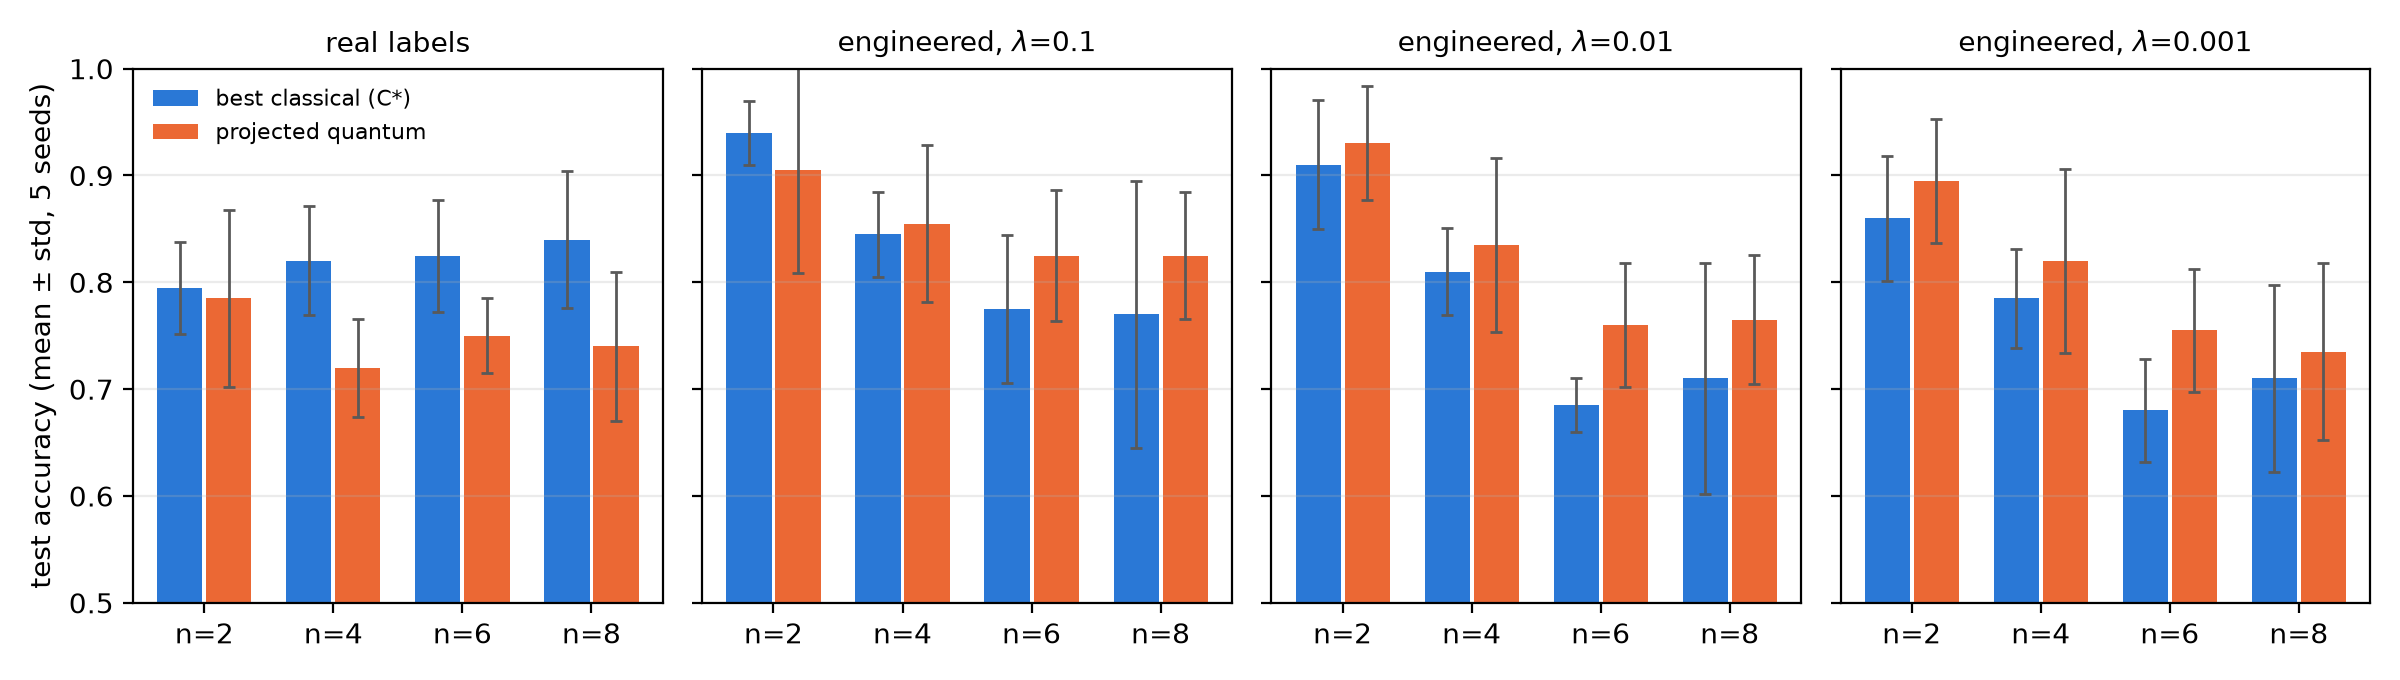
\includegraphics[width=\textwidth]{best_classical_vs_quantum.png}
\caption{Best classical model ($C^\ast$, chosen by training CV) vs.\ the projected quantum kernel (sampled), test accuracy, mean $\pm$ std over 5 seeds. Left: original labels. Right three panels: engineered labels for the three generator values of $\lambda$.}
\label{fig:bars}
\end{figure*}

\subsection{Geometric difference}

\begin{table}[t]
\centering
\caption{$g_{\mathrm{gen}}$ at $\lambda=0.1$ (training images, ideal quantum kernels), mean over 5 seeds.}
\label{tab:g}
\footnotesize
\begin{tabular}{@{}lcccc@{}}
\toprule
Pair & $n=2$ & $n=4$ & $n=6$ & $n=8$ \\
\midrule
Projected vs.\ RBF & 2.68 & 2.95 & 3.23 & 3.01 \\
Projected vs.\ polynomial & 2.88 & 2.97 & 3.49 & 4.15 \\
Projected vs.\ linear$^{a}$ & 0.64 & 0.96 & 0.90 & 1.21 \\
Projected vs.\ $C^\ast$ & 3.02 & 2.95 & 3.56 & 3.19 \\
\midrule
Fidelity vs.\ RBF & 2.61 & 2.83 & 2.45 & 2.35 \\
Fidelity vs.\ polynomial & 2.90 & 2.80 & 3.89 & 3.90 \\
Fidelity vs.\ linear$^{a}$ & 0.57 & 0.94 & 1.24 & 1.28 \\
Fidelity vs.\ $C^\ast$ & 2.87 & 2.83 & 3.54 & 2.81 \\
\bottomrule
\end{tabular}
\\[2pt]{\footnotesize $^{a}$Not comparable: the linear kernel has rank at most $n$, and its $g_{\mathrm{tra}}$ is 2.96--7.47, so the regularisation dominates.}
\end{table}

Table~\ref{tab:g} gives $g_{\mathrm{gen}}$ for all six pairs. Against the RBF, polynomial and $C^\ast$ kernels, $g_{\mathrm{gen}}$ lies between 2.35 and 4.15 for both quantum kernels, with no clear trend in $n$ over 2--8 qubits. The small values against the linear kernel are an artifact of regularisation: the linear kernel matrix has rank at most $n$, and its $g_{\mathrm{tra}}$ (2.96--7.47) is far above the other pairs (0.35--1.99). The value of $g_{\mathrm{gen}}$ depends on $\lambda$: for the pair with $C^\ast$, mean $g_{\mathrm{gen}}$ is 9.4--24.3 (projected) and 4.5--16.7 (fidelity) at $\lambda=10^{-3}$, and 1.2--1.9 at $\lambda=1$. Huang's rule ($g_{\mathrm{tra}}\le0.045$) can be met in only 15 of 60 projected pairs and 27 of 60 fidelity pairs (seed $\times$ $n$ $\times$ classical kernel).

Fig.~\ref{fig:dAg} plots $\Delta A$ against $g_{\mathrm{gen}}(K^{C^\ast}\|K^Q)$ for every seed and $n$. Since $C^\ast$ can be a different classical kernel in different seeds, the $C^\ast$ rows of Table~\ref{tab:g} average over kernel families; they measure the distance to the empirically selected classical model, not to one fixed kernel. There is no visible association: the correlation coefficient over the 20 points is $r=0.12$ for the projected kernel and $r=-0.01$ for the fidelity kernel. $\Delta A$ is positive in 3 of 20 projected runs and 7 of 20 fidelity runs (4 more are ties).

\begin{figure}[t]
\centering
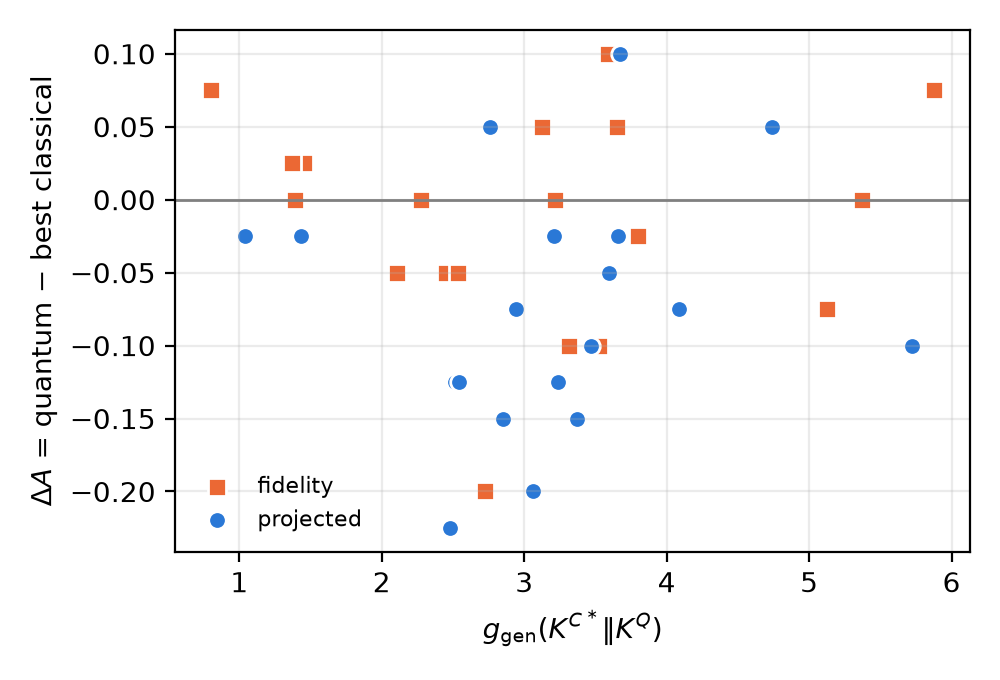
\includegraphics[width=\columnwidth]{deltaA_vs_g_original.png}
\caption{Original labels: accuracy gap $\Delta A$ vs.\ $g_{\mathrm{gen}}(K^{C^\ast}\|K^Q)$ at $\lambda=0.1$, one point per seed and qubit count.}
\label{fig:dAg}
\end{figure}

\subsection{Engineered labels}

\begin{table}[t]
\centering
\caption{Engineered labels: $\Delta A$ (sampled quantum kernel minus $C^\ast$), mean $\pm$ std over 5 seeds. $^\dagger$Meets the improvement criterion $\overline{\Delta A}>\sigma_{\Delta A}$.}
\label{tab:eng}
\scriptsize
\setlength{\tabcolsep}{2.5pt}
\begin{tabular}{@{}lcccc@{}}
\toprule
$\lambda$ & $n=2$ & $n=4$ & $n=6$ & $n=8$ \\
\midrule
\multicolumn{5}{@{}l}{\textit{Projected kernel}} \\
0.1 & $-0.035\pm0.072$ & $+0.010\pm0.041$ & $+0.050\pm0.035^\dagger$ & $+0.055\pm0.086$ \\
0.01 & $+0.020\pm0.040$ & $+0.025\pm0.052$ & $+0.075\pm0.057^\dagger$ & $+0.055\pm0.080$ \\
0.001 & $+0.035\pm0.051$ & $+0.035\pm0.049$ & $+0.075\pm0.050^\dagger$ & $+0.025\pm0.099$ \\
\midrule
\multicolumn{5}{@{}l}{\textit{Fidelity kernel}} \\
0.1 & $-0.035\pm0.075$ & $-0.015\pm0.025$ & $-0.065\pm0.060$ & $\phantom{+}0.000\pm0.079$ \\
0.01 & $-0.085\pm0.109$ & $+0.015\pm0.060$ & $+0.005\pm0.060$ & $-0.045\pm0.037$ \\
0.001 & $-0.010\pm0.041$ & $-0.005\pm0.037$ & $-0.030\pm0.029$ & $-0.040\pm0.034$ \\
\bottomrule
\end{tabular}
\end{table}

The engineered labels agree with the T-shirt/Shirt labels on 0.42--0.58 of the images (mean per $n$), so they define a new task on the same images. Classes are exactly balanced over the 120 images; on the fixed splits the training sets have 36--44 positive labels out of 80 and the test sets 16--24 out of 40. The engineered task is harder for the classical models: $C^\ast$ test accuracy falls from 0.940, 0.845, 0.775, 0.770 ($\lambda=0.1$) to 0.860, 0.785, 0.680, 0.710 ($\lambda=0.001$) for $n=2,4,6,8$, and logistic regression reaches only 0.565--0.770.

Table~\ref{tab:eng} and Fig.~\ref{fig:bars} (right panels) show that the projected kernel now has a positive mean gap in 11 of 12 settings, and meets the improvement criterion at $n=6$ for all three $\lambda$ ($+0.050$ to $+0.075$). At the other qubit counts the seed-to-seed spread is as large as the gap. The fidelity kernel, which the labels were not built for, shows no improvement in any setting. Fig.~\ref{fig:dAeng} compares the gaps with the original labels.

\begin{figure}[t]
\centering
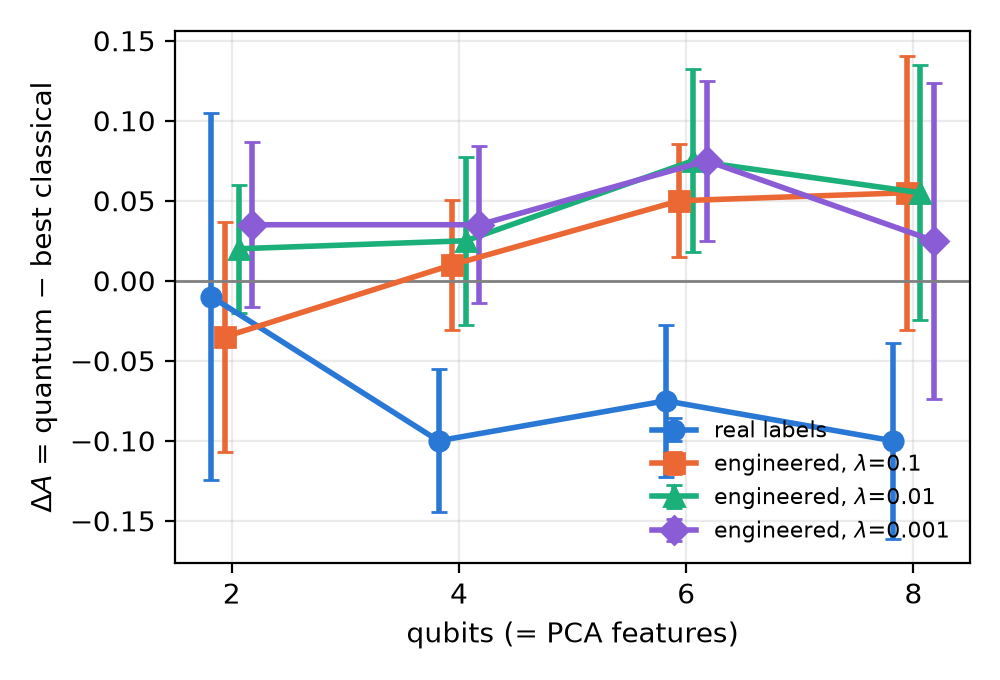
\includegraphics[width=\columnwidth]{deltaA_real_vs_engineered.png}
\caption{$\Delta A$ (projected, sampled, minus $C^\ast$) on the original and engineered labels, mean $\pm$ std over 5 seeds.}
\label{fig:dAeng}
\end{figure}

\subsection{Noise}

\begin{table*}[t]
\centering
\caption{Original labels: test accuracy of each quantum kernel at three levels (mean over 5 seeds), $\Delta A=A^Q_{\mathrm{noisy}}-A^{C^\ast}$ (mean $\pm$ std), and $g_{\mathrm{gen}}$ vs.\ $C^\ast$ from ideal and noisy kernels.}
\label{tab:noise}
\footnotesize
\setlength{\tabcolsep}{6pt}
\begin{tabular}{@{}lcccc@{}}
\toprule
 & $n=2$ & $n=4$ & $n=6$ & $n=8$ \\
\midrule
\multicolumn{5}{@{}l}{\textit{Projected kernel}} \\
Exact & 0.820 & 0.740 & 0.790 & 0.740 \\
Sampled & 0.785 & 0.720 & 0.750 & 0.740 \\
Noisy model & 0.790 & 0.720 & 0.750 & 0.725 \\
$\Delta A$ noisy & $-0.005\pm0.103$ & $-0.100\pm0.035$ & $-0.075\pm0.057$ & $-0.115\pm0.056$ \\
$g_{\mathrm{gen}}$ ideal / noisy & 3.02/2.98 & 2.95/2.92 & 3.56/3.54 & 3.19/3.15 \\
\midrule
\multicolumn{5}{@{}l}{\textit{Fidelity kernel}} \\
Exact & 0.830 & 0.795 & 0.795 & 0.845 \\
Sampled & 0.830 & 0.790 & 0.790 & 0.810 \\
Noisy model & 0.825 & 0.800 & 0.780 & 0.795 \\
$\Delta A$ noisy & $+0.030\pm0.048$ & $-0.020\pm0.033$ & $-0.045\pm0.053$ & $-0.045\pm0.076$ \\
$g_{\mathrm{gen}}$ ideal / noisy & 2.87/2.58 & 2.83/2.56 & 3.54/3.18 & 2.81/2.46 \\
\bottomrule
\end{tabular}
\end{table*}

Table~\ref{tab:noise} compares exact, sampled and noisy kernels. Moving from sampled to noisy changes mean test accuracy by between $-0.015$ and $+0.010$ for both kernels; most of the gap to the exact kernel is already present with finite shots alone. Neither kernel meets the improvement criterion over $C^\ast$ under noise (Table~\ref{tab:noise}, $\Delta A$ rows): the only positive mean gap, $+0.030\pm0.048$ for the fidelity kernel at $n=2$, is smaller than its spread.

The noise is visible in the kernel inputs. For the projected kernel, the mean absolute error of the Pauli features against exact values rises from 0.014--0.016 (sampled) to 0.030--0.079 (noisy), and the mean Bloch-vector length shrinks (e.g.\ 0.919 to 0.753 at $n=2$, 0.543 to 0.496 at $n=8$), as expected when noise pushes states towards the maximally mixed state. $\langle Y_k\rangle$ stays within 0.001 of zero on average, so the model shows no sign of coherent errors that would rotate the state out of its real-amplitude plane. For the fidelity kernel, the mean absolute error against the exact kernel rises from 0.006 (sampled) to 0.093--0.132 (noisy), and the mean off-diagonal value drops (0.745 to 0.641 at $n=2$). The smallest eigenvalue of the noisy fidelity matrix is $-0.048$ at $n=2$ and positive at $n\ge4$ (0.020--0.146); no repair is applied.

\textbf{Enhancement: noisy geometric difference.} Huang \textit{et al.} compute $g$ from ideal kernels. We also compute it from the noisy kernels (Table~\ref{tab:noise}). Noise lowers $g_{\mathrm{gen}}$ by 9--13\% for the fidelity kernel (mean ratio noisy/ideal 0.87--0.91 per $n$) but by only 0.5--1.4\% for the projected kernel (0.986--0.995). The projected kernel's geometry relative to the classical kernels is thus more robust to device noise in this setting.


\subsection{Discussion}\label{sec:disc}
\textbf{Original labels (sub-question 1).} Under a matched budget, neither quantum kernel shows an improvement over $C^\ast$ at any qubit count, so falsifier (ii) is not triggered (although, as discussed below, $g$ on these labels is not small). The $L=2$ fidelity kernel does not exceed its classically computable $L=1$ version except by one test image at $n=2$, and the projected kernel is below $C^\ast$ at every $n$. With 40 test images, differences below 0.025 correspond to less than one image per seed.

\textbf{Geometric difference (sub-question 2).} On the original labels $g_{\mathrm{gen}}\approx3$ for both kernels against $C^\ast$, i.e.\ the quantum kernels are geometrically different from the classical ones, yet there is no advantage and $\Delta A$ is not associated with $g$ across seeds and qubit counts. This is consistent with Huang \textit{et al.}: a large $g$ makes an advantage \emph{possible} for some labels; it does not guarantee one for a given task. $g$ shows no clear trend with $n$ over 2--8 qubits.

\textbf{Engineered labels (sub-question 3).} Because $g$ depends only on the images and kernels, the engineered task has the same $g$ as the original task (up to the change in tuned $C^\ast$); what differs is that the labels point along the direction where the projected kernel differs most from the classical kernels. Read literally, the Week~1 falsifier therefore leaves (i) \emph{untested}: no setting with a clearly larger $g$ exists, because relabeling cannot change $g$. Read as intended in Huang \textit{et al.}'s construction, i.e.\ labels aligned with the large-$g$ direction, (i) is tested and not triggered: on these labels the projected kernel meets the improvement criterion at $n=6$ for all three $\lambda$ and has a positive mean gap in 11 of 12 settings, while the fidelity kernel, whose geometry was not used, shows none. We report both readings. The gaps are small (0.050--0.075 at $n=6$) and have seed-to-seed spreads of the same size at the other qubit counts, and the generator was chosen after one preliminary check (Section~\ref{sec:changes}); with 5 seeds and 40 test images we treat this as weak evidence, not as a demonstrated advantage.

\textbf{Shots and noise (sub-question 4).} 2048 shots suffice for the fidelity kernel at $n=4$. The \texttt{ibm\_kingston} noise model shrinks the 1-RDM Bloch vectors and lowers fidelity-kernel values, but changes test accuracy by at most 0.015. Noise reduces the fidelity kernel's $g$ by about 10\% and leaves the projected kernel's $g$ almost unchanged.

\textbf{Limitations.} 80/40 images per seed, 5 seeds and a heuristic (not statistical) improvement criterion; one encoding circuit; noise from one calibration snapshot, with the noisy fidelity diagonal set to 1; engineered labels defined transductively on train and test images. All conclusions hold only for these models, budgets and data, not for quantum kernels in general.

\section{Changes since Week 1}\label{sec:changes}
\begin{itemize}
\item \textbf{Matched tuning budget.} The classical grids were changed to the budget in Table~\ref{tab:budget}. For seed 0, $n=4$, this changed one Week~1 number: the polynomial SVM now selects degree 5 and scores 0.850 accuracy and 0.920 AUC (Week~1: 0.825 and 0.923). All other Week~1 values and the choice $C^\ast=$ RBF are unchanged.
\item \textbf{Regularisation of $g$.} The Week~1 plan replaced $(K^C)^{-1}$ in Eq.~4 by $(K^C+\lambda I)^{-1}$ and chose the smallest $\lambda$ that keeps the condition number of $K^C+\lambda I$ below $10^8$. With 2--8 features both that rule and Huang's $g_{\mathrm{tra}}$ rule give values of $g$ that grow like $1/\sqrt{\lambda}$ and reflect the regulariser rather than the data (see the $\lambda$ values above). We therefore replace this form with Huang's $g_{\mathrm{gen}}$ (Eq.~5) at one fixed $\lambda=0.1$, chosen before any comparison with accuracy, and report the $\lambda$ dependence. This choice was made on a stand-in dataset before the project data were used.
\item \textbf{Engineered-label generator.} The Week~1 plan used a single fixed RBF kernel as $K^C$. A preliminary check (5 seeds, $n=4,6$) showed that labels built against one RBF kernel at $\lambda=0.1$ were easy for the tuned classical SVMs, which can choose other kernels. We replaced it with the sum of all 9 classical grid kernels and report three values of $\lambda$; this choice was informed by that check. The eigenvector is also taken from a different matrix than planned: the $g_{\mathrm{gen}}$ matrix of Eq.~5 instead of the Week~1 form $(K^{Q})^{1/2}(K^{C}+\lambda I)^{-1}(K^{Q})^{1/2}$, so that the labels follow the same quantity that we report as $g$.
\item \textbf{Code fix.} A cache in the fidelity code could reuse a transpiled circuit across qubit counts in one session. It was fixed before the Week~2 runs; Week~1 used a single qubit count and is unaffected.
\item \textbf{Reproducibility.} Re-running the projected-kernel notebook on Linux changed one seed's selected setting at $n=4$, because shot sampling differs slightly between platforms. All reported numbers come from one machine (Windows, Python 3.13.7, Qiskit 2.6.2) and are saved in the repository.
\end{itemize}

\section*{Status and Remaining Work}
\textbf{Done (Weeks 1--2):} data pipeline and saved splits for 5 seeds; classical baselines under a matched budget, with leakage check; fidelity kernel ($L=1$, $L=2$, sampled and exact) and projected kernel over 5 seeds and 2--8 qubits; shot study; geometric difference for all six pairs with $\lambda$ sensitivity; engineered labels; \texttt{ibm\_kingston} noise model with noisy $g$; all code and results on GitHub.

\textbf{Week 3 (Nov 29):} IBM hardware estimation of $\langle X_k\rangle$, $\langle Y_k\rangle$, $\langle Z_k\rangle$ for about 10 test samples and the four-level comparison (exact, sampled, noisy model, hardware); final $g$-vs-accuracy analysis.

\textbf{Week 4 (Dec 6):} final report and presentation; README with reproduction steps; tagged GitHub release.

\section*{Author Contributions}
F.~Shahzad: shared data and evaluation code, encoding circuit, fidelity kernel, qubit and shot studies, IBM hardware run. S.~ul~Arifeen: projected-kernel features and kernel, noise model and noisy geometric difference, simulator--hardware comparison. H.~Nadeem: classical baselines and matched budget, geometric difference, engineered dataset, final $g$-vs-accuracy analysis. All authors contribute to the report and presentation.

\begin{thebibliography}{4}
\bibitem{huang2021} H.-Y. Huang, M. Broughton, M. Mohseni, R. Babbush, S. Boixo, H. Neven, and J. R. McClean, ``Power of data in quantum machine learning,'' \textit{Nat. Commun.}, vol. 12, p. 2631, 2021.
\bibitem{schuld2019} M. Schuld and N. Killoran, ``Quantum machine learning in feature Hilbert spaces,'' \textit{Phys. Rev. Lett.}, vol. 122, p. 040504, 2019.
\bibitem{havlicek2019} V. Havl\'{i}\v{c}ek \textit{et al.}, ``Supervised learning with quantum-enhanced feature spaces,'' \textit{Nature}, vol. 567, pp. 209--212, 2019.
\bibitem{xiao2017} H. Xiao, K. Rasul, and R. Vollgraf, ``Fashion-MNIST: a novel image dataset for benchmarking machine learning algorithms,'' arXiv:1708.07747, 2017.
\end{thebibliography}

\end{document}
